  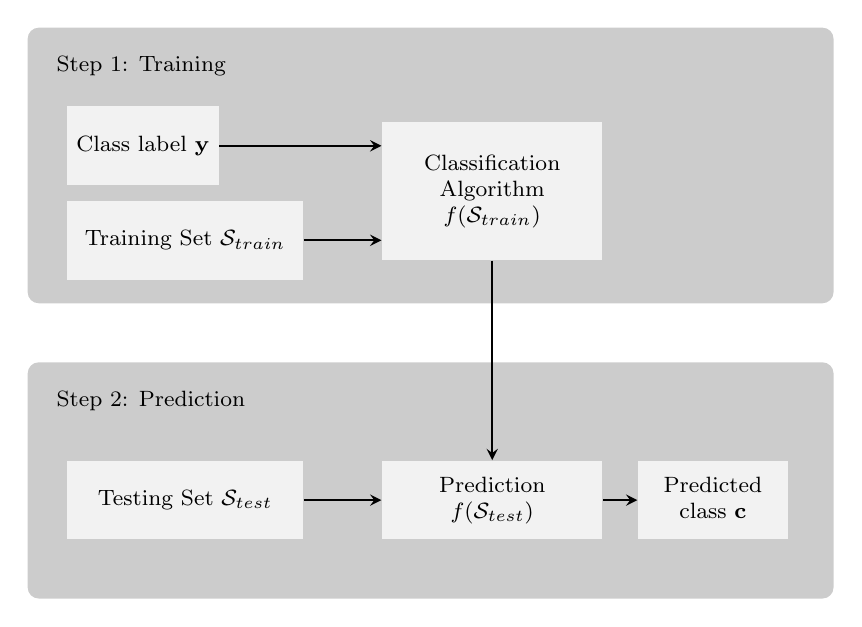
\begin{tikzpicture}[node distance=2cm]
  \tikzstyle{every node}=[font=\footnotesize]
  
  % Main boxes
  \node (step1) [rectangle, rounded corners, anchor=north west, fill=black!20, text width=10cm,
								minimum height=3.5cm] {};
	\node [anchor=north west, yshift=-0.25cm, xshift=0.25cm] at (step1.north west){Step 1: Training};
	\node (step2) [rectangle, rounded corners, anchor=west, fill=black!20, text width=10cm, 
								minimum height=3cm, below of = step1, yshift=-2cm] {};
	\node [anchor=north west, yshift=-0.25cm, xshift=0.25cm] at (step2.north west){Step 2: 
                Prediction};
	
	% Training
	\node (label) [rectangle, anchor=north west, fill=black!5, minimum height=1cm,
								yshift=-1cm, xshift=0.5cm] {Class label $\bf y $};
	\node (train) [rectangle, anchor=north west, fill=black!5, minimum height=1cm, minimum width=3cm,
								yshift=-2.2cm, xshift=0.5cm] {Training Set $\mathcal{S}_{train} $};
	\node (algo) [rectangle, anchor=north west, fill=black!5, minimum height=1.75cm,
							 minimum width=2.8cm, yshift=-1.2cm, xshift=4.5cm] 
							 {\tabular{c} Classification \\ Algorithm  \\	$f(\mathcal{S}_{train}) $
								\endtabular}; 

	%Classification
	\node (test) [rectangle, anchor=north west, fill=black!5, minimum height=1cm, minimum width=3cm,
								yshift=-5.5cm, xshift=0.5cm] {Testing Set $\mathcal{S}_{test} $};
	\node (algo2)[rectangle, anchor=north west, fill=black!5, minimum height=1cm, minimum width=2.8cm,
							 yshift=-5.5cm, xshift=4.5cm] 
							 {\tabular{c} Prediction \\	$f(\mathcal{S}_{test}) $\endtabular};
	\node (pred) [rectangle, anchor=north west, fill=black!5, minimum height=1cm,
							yshift=-5.5cm, xshift=7.75cm] {\tabular{c} Predicted \\ class $\bf c$	\endtabular};
	
	% Arrows
	\node (label_temp) [rectangle, anchor=north west, minimum height=1cm, yshift=-1cm, 
                xshift=4.5cm] {};
	\draw[thick,->,>=stealth] (label) to (label_temp);
	\node (train_temp) [rectangle, anchor=north west,minimum height=1cm, minimum width=3cm,
								yshift=-2.2cm, xshift=4.5cm] {};
	\draw[thick,->,>=stealth] (train) to (train_temp);
	\draw[thick,->,>=stealth] (algo) to (algo2);
	\draw[thick,->,>=stealth] (test) to (algo2);
	\draw[thick,->,>=stealth] (algo2) to (pred);
  \end{tikzpicture}
 